\documentclass[AMA,STIX1COL,]{WileyNJD-v2}
% examples/header.tex
\usepackage{amsthm}


% Pandoc syntax highlighting
\usepackage{color}
\usepackage{fancyvrb}
\newcommand{\VerbBar}{|}
\newcommand{\VERB}{\Verb[commandchars=\\\{\}]}
\DefineVerbatimEnvironment{Highlighting}{Verbatim}{commandchars=\\\{\}}
% Add ',fontsize=\small' for more characters per line
\usepackage{framed}
\definecolor{shadecolor}{RGB}{248,248,248}
\newenvironment{Shaded}{\begin{snugshade}}{\end{snugshade}}
\newcommand{\AlertTok}[1]{\textcolor[rgb]{0.94,0.16,0.16}{#1}}
\newcommand{\AnnotationTok}[1]{\textcolor[rgb]{0.56,0.35,0.01}{\textbf{\textit{#1}}}}
\newcommand{\AttributeTok}[1]{\textcolor[rgb]{0.77,0.63,0.00}{#1}}
\newcommand{\BaseNTok}[1]{\textcolor[rgb]{0.00,0.00,0.81}{#1}}
\newcommand{\BuiltInTok}[1]{#1}
\newcommand{\CharTok}[1]{\textcolor[rgb]{0.31,0.60,0.02}{#1}}
\newcommand{\CommentTok}[1]{\textcolor[rgb]{0.56,0.35,0.01}{\textit{#1}}}
\newcommand{\CommentVarTok}[1]{\textcolor[rgb]{0.56,0.35,0.01}{\textbf{\textit{#1}}}}
\newcommand{\ConstantTok}[1]{\textcolor[rgb]{0.00,0.00,0.00}{#1}}
\newcommand{\ControlFlowTok}[1]{\textcolor[rgb]{0.13,0.29,0.53}{\textbf{#1}}}
\newcommand{\DataTypeTok}[1]{\textcolor[rgb]{0.13,0.29,0.53}{#1}}
\newcommand{\DecValTok}[1]{\textcolor[rgb]{0.00,0.00,0.81}{#1}}
\newcommand{\DocumentationTok}[1]{\textcolor[rgb]{0.56,0.35,0.01}{\textbf{\textit{#1}}}}
\newcommand{\ErrorTok}[1]{\textcolor[rgb]{0.64,0.00,0.00}{\textbf{#1}}}
\newcommand{\ExtensionTok}[1]{#1}
\newcommand{\FloatTok}[1]{\textcolor[rgb]{0.00,0.00,0.81}{#1}}
\newcommand{\FunctionTok}[1]{\textcolor[rgb]{0.00,0.00,0.00}{#1}}
\newcommand{\ImportTok}[1]{#1}
\newcommand{\InformationTok}[1]{\textcolor[rgb]{0.56,0.35,0.01}{\textbf{\textit{#1}}}}
\newcommand{\KeywordTok}[1]{\textcolor[rgb]{0.13,0.29,0.53}{\textbf{#1}}}
\newcommand{\NormalTok}[1]{#1}
\newcommand{\OperatorTok}[1]{\textcolor[rgb]{0.81,0.36,0.00}{\textbf{#1}}}
\newcommand{\OtherTok}[1]{\textcolor[rgb]{0.56,0.35,0.01}{#1}}
\newcommand{\PreprocessorTok}[1]{\textcolor[rgb]{0.56,0.35,0.01}{\textit{#1}}}
\newcommand{\RegionMarkerTok}[1]{#1}
\newcommand{\SpecialCharTok}[1]{\textcolor[rgb]{0.00,0.00,0.00}{#1}}
\newcommand{\SpecialStringTok}[1]{\textcolor[rgb]{0.31,0.60,0.02}{#1}}
\newcommand{\StringTok}[1]{\textcolor[rgb]{0.31,0.60,0.02}{#1}}
\newcommand{\VariableTok}[1]{\textcolor[rgb]{0.00,0.00,0.00}{#1}}
\newcommand{\VerbatimStringTok}[1]{\textcolor[rgb]{0.31,0.60,0.02}{#1}}
\newcommand{\WarningTok}[1]{\textcolor[rgb]{0.56,0.35,0.01}{\textbf{\textit{#1}}}}

% tightlist command for lists without linebreak
\providecommand{\tightlist}{%
  \setlength{\itemsep}{0pt}\setlength{\parskip}{0pt}}


% Pandoc citation processing
\newlength{\cslhangindent}
\setlength{\cslhangindent}{1.5em}
\newlength{\csllabelwidth}
\setlength{\csllabelwidth}{3em}
\newlength{\cslentryspacingunit} % times entry-spacing
\setlength{\cslentryspacingunit}{\parskip}
% for Pandoc 2.8 to 2.10.1
\newenvironment{cslreferences}%
  {}%
  {\par}
% For Pandoc 2.11+
\newenvironment{CSLReferences}[2] % #1 hanging-ident, #2 entry spacing
 {% don't indent paragraphs
  \setlength{\parindent}{0pt}
  % turn on hanging indent if param 1 is 1
  \ifodd #1
  \let\oldpar\par
  \def\par{\hangindent=\cslhangindent\oldpar}
  \fi
  % set entry spacing
  \setlength{\parskip}{#2\cslentryspacingunit}
 }%
 {}
\usepackage{calc}
\newcommand{\CSLBlock}[1]{#1\hfill\break}
\newcommand{\CSLLeftMargin}[1]{\parbox[t]{\csllabelwidth}{#1}}
\newcommand{\CSLRightInline}[1]{\parbox[t]{\linewidth - \csllabelwidth}{#1}\break}
\newcommand{\CSLIndent}[1]{\hspace{\cslhangindent}#1}


\articletype{Research article}

\received{2017-01-01}

\revised{2017-02-01}

\accepted{2017-03-01}

\raggedbottom

\begin{document}


\title{A demonstration of the \LaTeX class file for Statistics in
Medicine with Rmarkdown}

\author[a,b]{A. Uthor*}
\author[b]{O. Tro}
\author[c]{O. Vriga}

\authormark{Uthor \emph{et al}.}

\address[a]{Department of Incredible Research, University A, City A,
Country A}
\address[b]{Department of Applied Things, University B, City B, Country
B}
\address[c]{Very Important Stuff Committee, Institute C, City C, Country
C}

\corres{*Corresponding author name, This is sample corresponding
address. \email{authorone@gmail.com}}

\presentaddress{This is sample for present address text this is sample
for present address text}

\abstract{Lorem ipsum dolor sit amet, consectetur adipiscing elit.
Aenean ut elit odio. Donec fermentum tellus neque, vitae fringilla orci
pretium vitae. Fusce maximus finibus facilisis. Donec ut ullamcorper
turpis. Donec ut porta ipsum. Nullam cursus mauris a sapien ornare
pulvinar. Aenean malesuada molestie erat quis mattis. Praesent
scelerisque posuere faucibus. Praesent nunc nulla, ullamcorper ut
ullamcorper sed, molestie ut est. Donec consequat libero nisi, non
semper velit vulputate et. Quisque eleifend tincidunt ligula, bibendum
finibus massa cursus eget. Curabitur aliquet vehicula quam non pulvinar.
Aliquam facilisis tortor nec purus finibus, sit amet elementum eros
sodales. Ut porta porttitor vestibulum. Integer molestie, leo ut maximus
aliquam, velit dui iaculis nibh, eget hendrerit purus risus sit amet
dolor. Sed sed tincidunt ex. Curabitur imperdiet egestas tellus in
iaculis. Maecenas ante neque, pretium vel nisl at, lobortis lacinia
neque. In gravida elit vel volutpat imperdiet. Sed ut nulla arcu. Proin
blandit interdum ex sit amet laoreet. Phasellus efficitur, sem hendrerit
mattis dapibus, nunc tellus ornare nisi, nec eleifend enim nibh ac
ipsum. Aenean tincidunt nisl sit amet facilisis faucibus. Donec odio
erat, bibendum eu imperdiet sed, gravida luctus turpis.}

\keywords{Class file; \LaTeX; Statist. Med.; Rmarkdown;}

\maketitle

\hypertarget{the-article-header-information}{%
\section{The Article Header
Information}\label{the-article-header-information}}

YAML header:

\begin{verbatim}
output:
  rticles::sim_article:
    keep_tex: TRUE
\end{verbatim}

Configure the YAML header including the following elements:

\begin{itemize}
\item
  \texttt{title}: Title
\item
  \texttt{author}: List of author(s) containing \texttt{name} and
  \texttt{num}
\item
  \texttt{address}: List containing \texttt{num} and \texttt{org} for
  defining \texttt{author} affiliations
\item
  \texttt{presentaddress}: Not sure what they mean with this
\item
  \texttt{corres}: Author and address for correspondence
\item
  \texttt{authormark}: Short author list for header
\item
  \texttt{received}, \texttt{revised}, \texttt{accepted}: dates of
  submission, revision, and acceptance of the manuscript
\item
  \texttt{abstract}: Limited to 250 words
\item
  \texttt{keywords}: Up to 6 keywords
\item
  \texttt{bibliography}: BibTeX \texttt{.bib} file
\item
  \texttt{classoption}: options of the \texttt{WileyNJD-v2} class
\item
  \texttt{longtable}: set to \texttt{true} to include the
  \texttt{longtable} package, used by default from \texttt{pandoc} to
  convert markdown to \LaTeX code
\end{itemize}

\hypertarget{remarks}{%
\subsection{Remarks}\label{remarks}}

\begin{enumerate}
\def\labelenumi{\arabic{enumi}.}
\item
  In \texttt{authormark} use \emph{et al.} if there are three or more
  authors.
\item
  Note the use of \texttt{num} to link names and addresses.
\item
  For submitting a double-spaced manuscript, add \texttt{doublespace} as
  an option to a \texttt{classoption} line in the YAML header:
  \texttt{classoption:\ doublespace}.
\item
  Keywords are separated by semicolons.
\end{enumerate}

\hypertarget{the-body-of-the-article}{%
\section{The Body of the Article}\label{the-body-of-the-article}}

\hypertarget{mathematics}{%
\subsection{Mathematics}\label{mathematics}}

Use mathematics in Rmarkdown as usual.

\hypertarget{figures-and-tables}{%
\subsection{Figures and Tables}\label{figures-and-tables}}

Figures are supported from R code:

\begin{Shaded}
\begin{Highlighting}[]
\NormalTok{x }\OtherTok{=} \FunctionTok{rnorm}\NormalTok{(}\DecValTok{10}\NormalTok{)}
\NormalTok{y }\OtherTok{=} \FunctionTok{rnorm}\NormalTok{(}\DecValTok{10}\NormalTok{)}
\FunctionTok{plot}\NormalTok{(x, y)}
\end{Highlighting}
\end{Shaded}

\begin{figure}
\centering
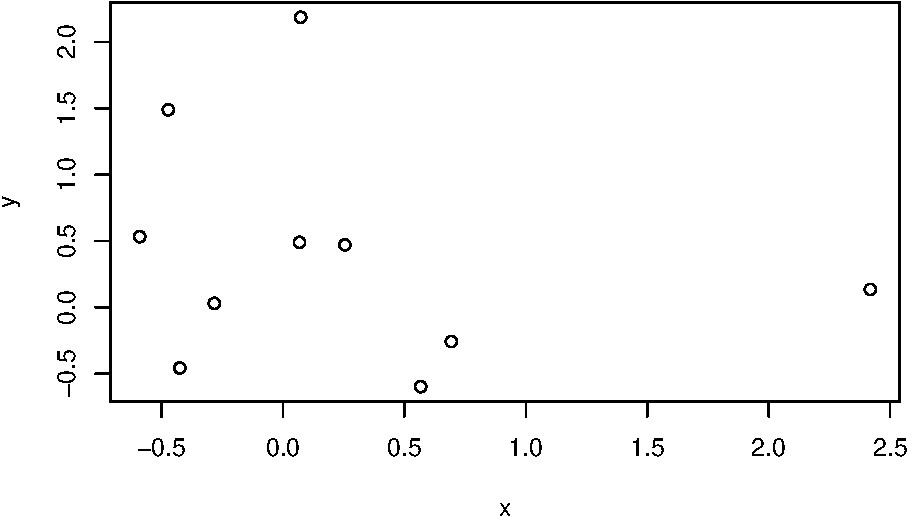
\includegraphics{article_files/figure-latex/plot-ref-1.pdf}
\caption{Fancy Caption\label{fig:plot}}
\end{figure}

\ldots and can be referenced (Figure \ref{fig:plot}) by including the
\texttt{\textbackslash{}\textbackslash{}label\{\}} tag in the
\texttt{fig.cap} attribute of the R chunk:
\texttt{fig.cap\ =\ "Fancy\ Caption\textbackslash{}\textbackslash{}label\{fig:plot\}"}.
It is a quirky hack at the moment, see
\href{https://github.com/yihui/knitr/issues/323}{here}.

Analogously, use Rmarkdown to produce tables as usual:

\begin{Shaded}
\begin{Highlighting}[]
\ControlFlowTok{if}\NormalTok{ (}\SpecialCharTok{!}\FunctionTok{require}\NormalTok{(}\StringTok{"xtable"}\NormalTok{)) }\FunctionTok{install.packages}\NormalTok{(}\StringTok{"xtable"}\NormalTok{)}
\end{Highlighting}
\end{Shaded}

\begin{verbatim}
## Loading required package: xtable
\end{verbatim}

\begin{Shaded}
\begin{Highlighting}[]
\NormalTok{xt }\OtherTok{\textless{}{-}} \FunctionTok{xtable}\NormalTok{(}\FunctionTok{head}\NormalTok{(cars), }\AttributeTok{caption =} \StringTok{"A table"}\NormalTok{, }\AttributeTok{label =} \StringTok{"tab:table"}\NormalTok{)}
\FunctionTok{print}\NormalTok{(xt, }\AttributeTok{comment =} \ConstantTok{FALSE}\NormalTok{)}
\end{Highlighting}
\end{Shaded}

\begin{table}[ht]
\centering
\begin{tabular}{rrr}
  \hline
 & speed & dist \\ 
  \hline
1 & 4.00 & 2.00 \\ 
  2 & 4.00 & 10.00 \\ 
  3 & 7.00 & 4.00 \\ 
  4 & 7.00 & 22.00 \\ 
  5 & 8.00 & 16.00 \\ 
  6 & 9.00 & 10.00 \\ 
   \hline
\end{tabular}
\caption{A table} 
\label{tab:table}
\end{table}

Referenced via \ref{tab:table}. You can also use the YAML option
\texttt{header-includes} to includes custom \LaTeX packages for tables
(keep in mind that \texttt{pandoc} uses \texttt{longtables} by default,
and it is hardcoded; some things may require including the package
\texttt{longtable}). E.g., using \texttt{ctable}:

\begin{verbatim}
header-includes:
- \usepackage{ctable}
\end{verbatim}

Then, just write straight-up \LaTeX code and reference is as usual
(\texttt{\textbackslash{}ref\{tab:ctable\}}):

\begin{verbatim}
\ctable[cap = {Short caption},
        caption = {A long, long, long, long, long caption for this table.},
        label={tab:ctable},]
        {cc}
        {
        \tnote[$\ast$]{Footnote 1}
        \tnote[$\dagger$]{Other footnote}
        \tnote[b]{Mistakes are possible.}
        }{
        \FL
        COL 1\tmark[a] & COL 2\tmark[$\ast$]
        \ML
        6.92\tmark[$\dagger$] & 0.09781 \\
        6.93\tmark[$\dagger$] & 0.09901 \\
        97 & 2000
        \LL
}
\end{verbatim}

It is also possible to set the \texttt{YAML} option
\texttt{longtable:\ true} and use markdown tables (or the
\texttt{knitr::kable} function): \texttt{knitr::kable(head(cars))}
produces the same table as the \texttt{xtable} example presented before.

\hypertarget{cross-referencing}{%
\subsection{Cross-referencing}\label{cross-referencing}}

The use of the Rmarkdown equivalent of the \LaTeX cross-reference system
for figures, tables, equations, etc., is encouraged (using
\texttt{{[}@\textless{}name\textgreater{}{]}}, equivalent of
\texttt{\textbackslash{}ref\{\textless{}name\textgreater{}\}} and
\texttt{\textbackslash{}label\{\textless{}name\textgreater{}\}}). That
works well for citations in Rmarkdown, not so well for figures and
tables. In that case, it is possible to revert to standard
\LaTeX syntax.

\hypertarget{double-spacing}{%
\subsection{Double Spacing}\label{double-spacing}}

If you need to double space your document for submission please use the
\texttt{doublespace} option in the header.

\hypertarget{bibliography}{%
\section{Bibliography}\label{bibliography}}

Link a \texttt{.bib} document via the YAML header, and bibliography will
be printed at the very end (as usual). The default bibliography style is
provided by Wiley as in \texttt{WileyNJD-AMA.bst}, do not delete that
file.

\begin{description}
\item[Lemma (Pumping Lemming). \label{pumping}]
Let \(L\) be a regular language. Then there exists an integer
\(p \geq 1\) called the ``pumping length'' which depends only on \(L\),
such that every string \(w \in L\) of length at least \(p\) can be
divided into three substrings \(w = xyz\) such that the following
conditions hold:

\begin{itemize}
\tightlist
\item
  \(|y| \geq 1\)
\item
  \(|xy| \leq p\)
\item
  \(xy^n z \in L\), for all \(n \geq 0\).
\end{itemize}

That is, the non-empty substring \(y\) occurring within the first \(p\)
characters of \(w\) can be ``pumped'' any number of times, and the
resulting string is always in \(L\).
\end{description}

Use the Rmarkdown equivalent of the \LaTeX citation system using
\texttt{{[}@\textless{}name\textgreater{}{]}}. Example: (Taylor and
Green 1937), (Knupp 1999; \textbf{Kamm2000?}).

To include all citation from the \texttt{.bib} file, add
\texttt{\textbackslash{}nocite\{*\}} before the end of the document.

\hypertarget{further-information}{%
\section{Further information}\label{further-information}}

All \LaTeX enviroments supported by the main template are supported here
as well; see the \texttt{.tex} sample file
\href{http://onlinelibrary.wiley.com/journal/10.1002/(ISSN)1097-0258/homepage/la_tex_class_file.htm}{here}
for more details and example.

\hypertarget{refs}{}
\begin{CSLReferences}{1}{0}
\leavevmode\vadjust pre{\hypertarget{ref-Knupp1999}{}}%
Knupp, PM. 1999. {``Winslow Smoothing on Two-Dimensional Unstructured
Meshes.''} \emph{Eng {C}omput} 15: 263--68.

\leavevmode\vadjust pre{\hypertarget{ref-Taylor1937}{}}%
Taylor, GI, and AE Green. 1937. {``Mechanism of the Production of Small
Eddies from Large Ones.''} \emph{P {R}oy {S}oc {L}ond {A} {M}at} 158
(895): 499--521.

\end{CSLReferences}

\bibliography{bibfile.bib}


\end{document}